\documentclass{astroedu-lab}

\begin{document}

\pagestyle{plain}

\begin{problem}{\huge Лабораторная работа 5.4.2\\\\Исследование энергетического\\\\спектра $\beta$-частиц\\\\Выполнил Жданов Елисей Б01-205}

\section{Цель работы:}

С помощью магнитного спектрометра исследовать энергетический спектр $\beta$-частиц при распаде ядер $^{137}$Cs и определить их максимальную энергию.


\section{Оборудование:}

Бета спектрометр

Вакуумная камера

\section{Теоретическая справка}

Бета-распад - самопроизвольное превращение ядер, при котором их массовое число не изменяется, а заряд увеличивается или уменьшается на единицу.
	В данной работе:
	$$^A_Z X \to ^{\ \, A}_{Z+1} X + e^- + \widetilde{\nu} .$$
	
	Величина $W(p_e)$ является плотностью вероятности. Распределение электронов по энергии может быть вычислено теоретически. Для разрешенных переходов вероятность $\beta$-распада просто попрорциональна сатистическому весу.
	\begin{equation*}
		\label{eq:W}
		W(p_e)dp_e \propto p_e^2(E_m-E_e)^2 dp_e.
	\end{equation*}
	Кинетическая энергия электрона и его импульс связаны друг с другом обычной формулой:
	\begin{equation*}
		E = \sqrt{(p_ec)^2+(m_ec^2)^2}-m_ec^2
	\end{equation*}
	Выражение (\ref{eq:W}) приводит к спектру, имеющему вид широкого колокола. Кривая плавно отходит от нулся и стольже плавно, по параболе, касается оси абсцисс в области максимального импульса электронов.
	
	Дочерние ядра, возникающие в результате $\beta$-распада, нередко оказываются возбужденными. Возбужденные ядра отдают свою энергию либо излучая $\gamma$-квант, либо передвавая избыток энергии одному из электронов внутренних оболочек атома. Излучаемые в таком процессе электроны имеют строго определенную энергию и называются \textit{конверсионными}.
	
	Конверсия чаще всего происходит на оболочках K и L. Ширина конверсионной линии является чисто аппаратурной -- по ней можно оценить разрешающую силу спектрометра.
	

\section{Экспериментальная установка}

Блок-схема установки для изучения $\beta$-спектров изображена на рис. Радиоактивный источник $^{137}$Cs помещен внутрь откачанной трубы. Электроны, сфокусированные магнитной линзой, попадают в счетчик. В газоразрядном счетчике они инициируют газовый разряд и тем самым приводят к появлению электрических импульсов на электродах, которые затем регистрируются пересчетным прибором.
	
	
\begin{figure}[!h]
	\centering
	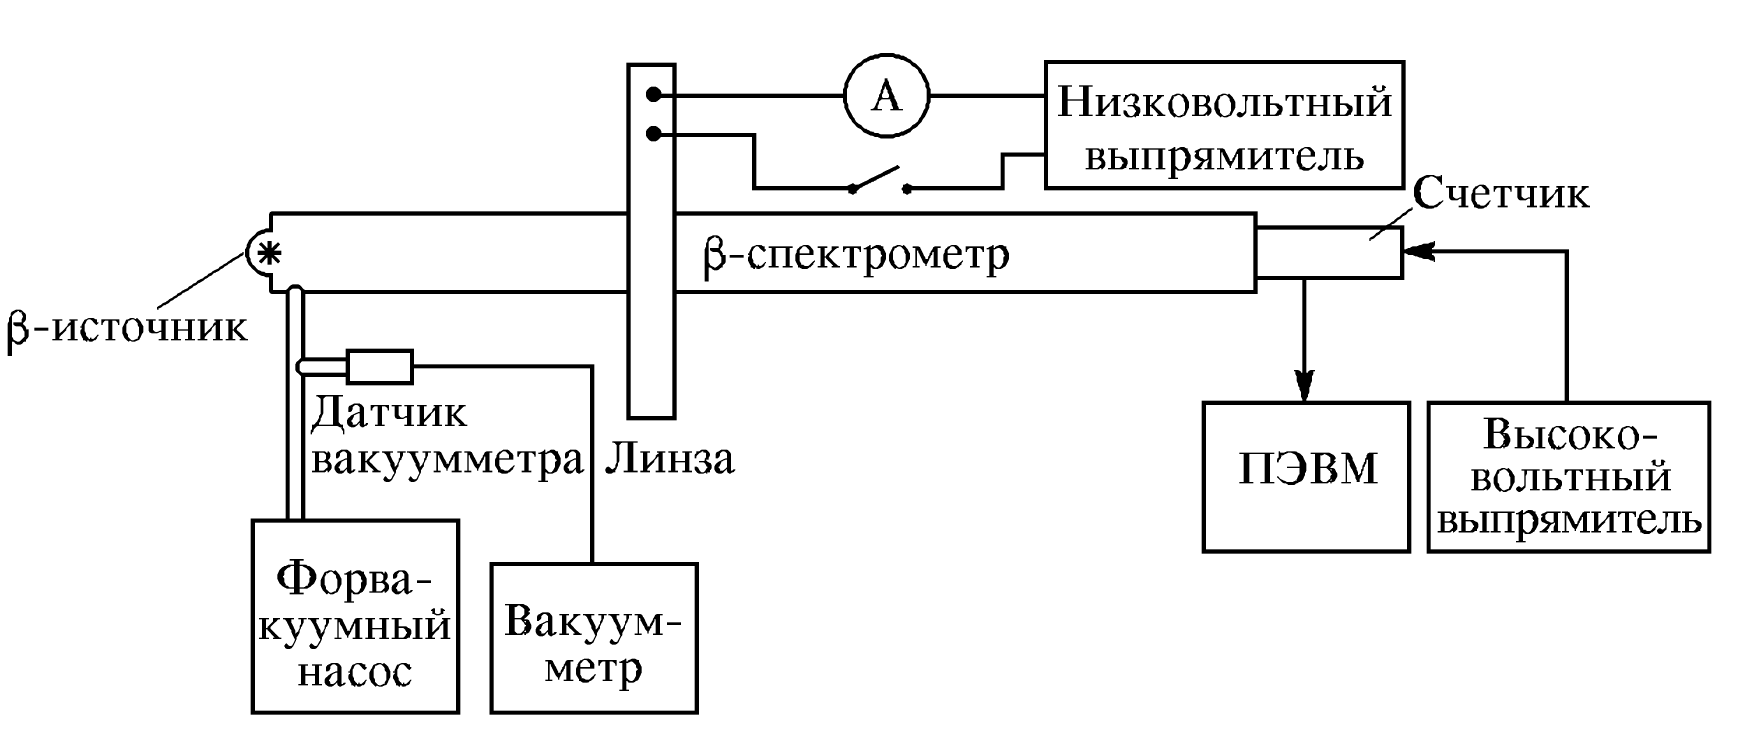
\includegraphics[width=1\textwidth]{shema.png}
	\label{fig:boiler}
\end{figure}
	

\begin{figure}[!h]
	\centering
	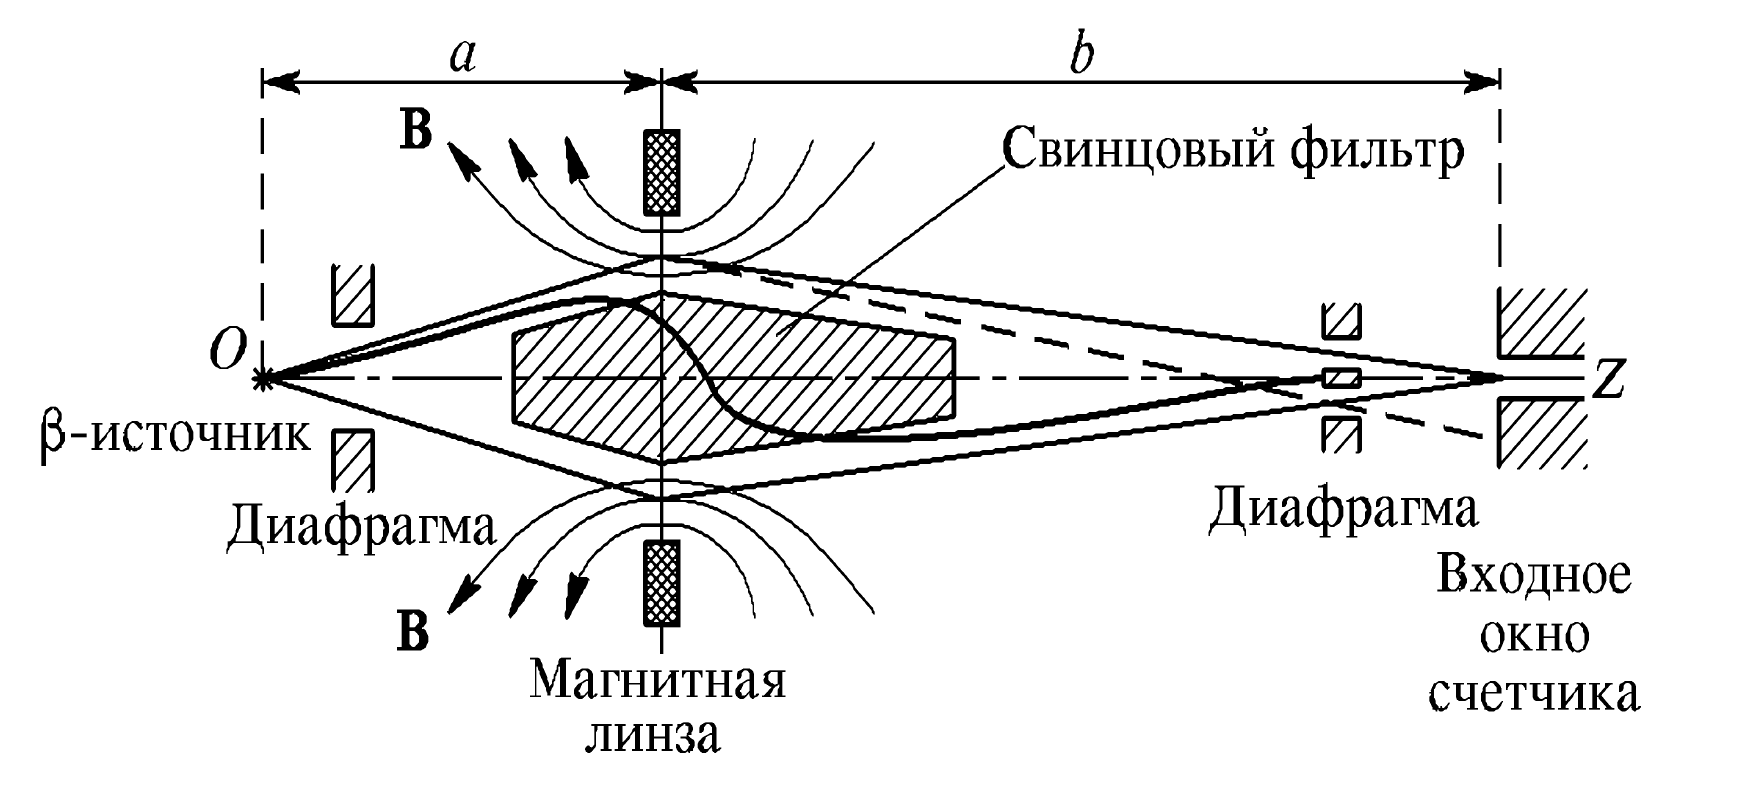
\includegraphics[width=1\textwidth]{ustanovka.png}
	\label{fig:boiler}
\end{figure}	
	

	Энергию $\beta$-частиц определяют с помощью $\beta$-спектрометров (рис.). В работе используется магнитный спектрометр с <<короткой линзой>>. Отметим, что в течение всего опыта геометрия прибора остается неизменной, поэтому импульс сфокусированных электронов пропорционален величине тока:
	\begin{equation}
		\label{eq:pkI}
		\tag{$\star$}
		p_e = kI.
	\end{equation}

	Cвязь между числом частиц, регистрируемых установкой, и функцией $W(p_e)$ выражается формулой:
	\begin{equation*}
		N(p_e) \propto W(p_e)p_e,
	\end{equation*}
	откуда
	\begin{equation}
		\label{eq:fermi}
		\tag{$\star \star$}
		\frac{\sqrt{N}}{p_e^{3/2}} \propto E_m - E
	\end{equation}
	
	

\section{Измерения, Обработка}




По результатам измерений построим график cпектра $\beta$-распада атома $^{137}$Cs и откалибруем его. Для этого пересчитаем значения силы тока в импульс по формуле (\ref{eq:pkI}). Коэффициент $k$ определим по известной конверсионной линии:
			$$kcI_0 = 1013.5 \ \text{кэВ},$$
		где $c$ -- скорость света, $I_0 = 3.25$ А -- сила тока, при которой наблюдается конверсионный пик. Получаем, что $$k = (312 \pm 2) \frac{\text{кэВ}}{c\cdot\text{А}}.$$
		
		Сдвиг графика по оси ординат сделаем на величину радиационного фона $N_\text{ф}$ при $I = 4.10$ А и $I = 0$ А, так как в этом случае график касается оси абсцисс в области максимальной энергии, что соответствует теоретической зависимости.
		

\begin{figure}[!h]
	\centering
	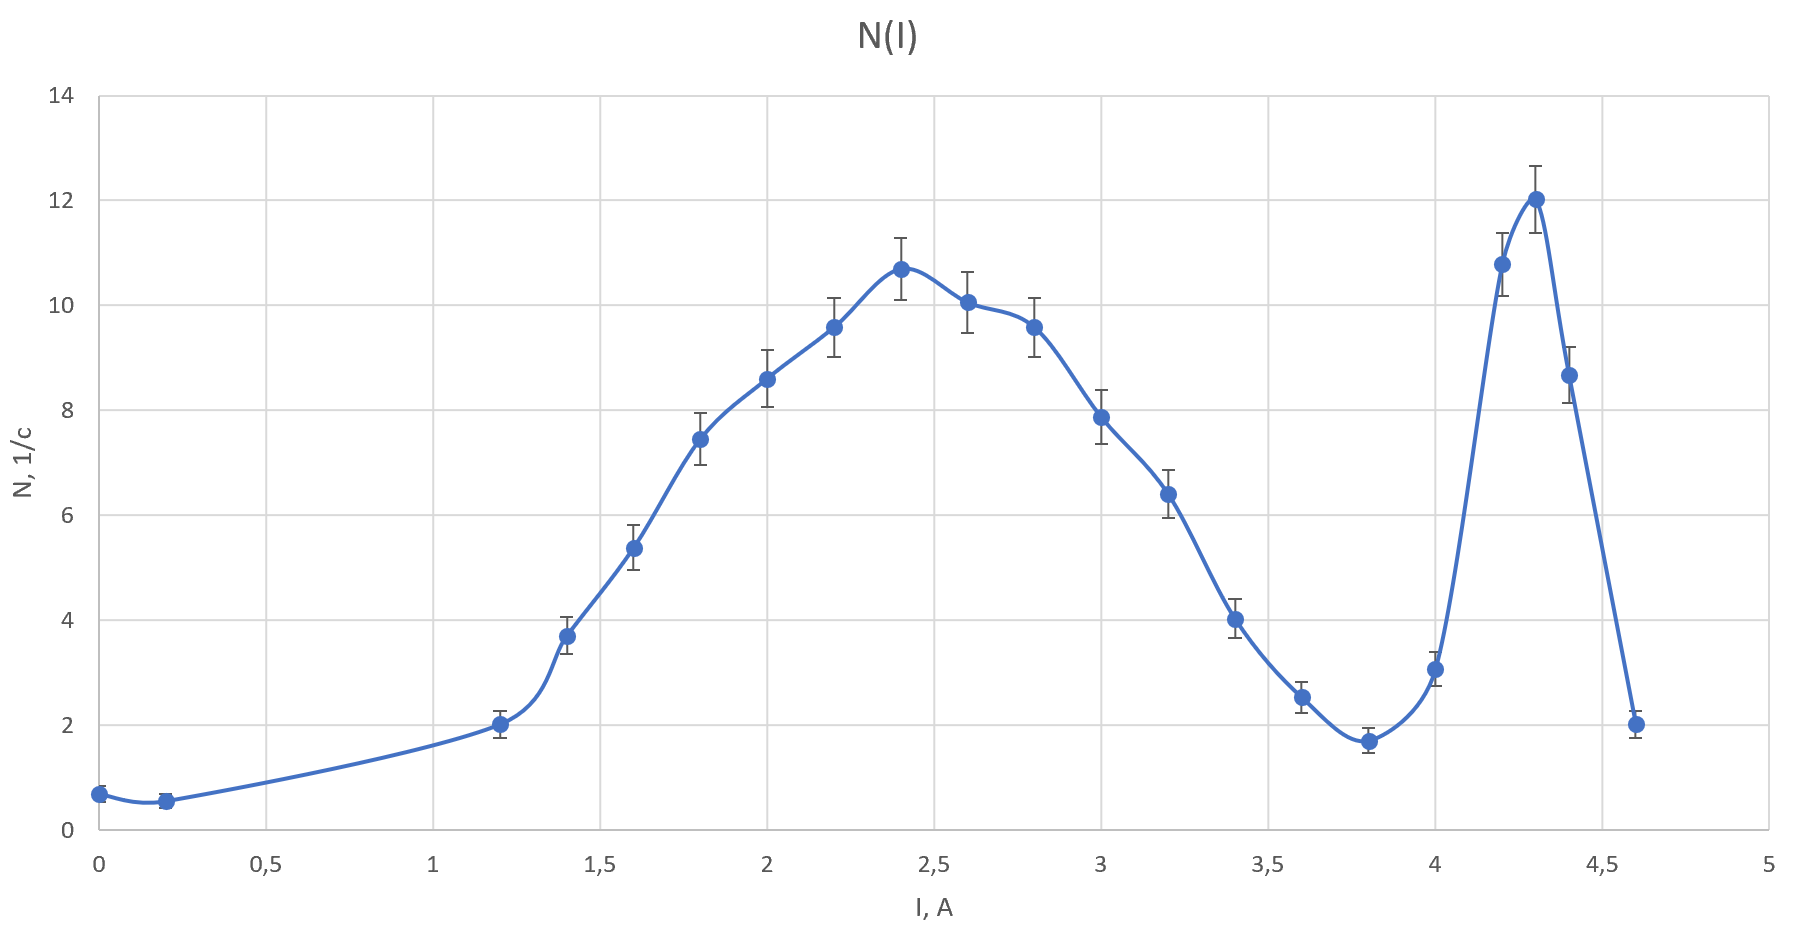
\includegraphics[width=1\textwidth]{doc.png}
	\label{fig:boiler}
\end{figure}			
		
		\newpage
		Определим максимальную энергию $\beta$-спектра. Анализ рис. в таком случае даст достаточно грубый результат, так как нам придётся ограничииться исследованием точек у самой верхней границы спектра. Эти точки измерены с наименьшей статистической точностью. Однако мы можем уменьшить ошибку определения максимальной энергии посредством процедуры Ферми-Кюри. Для этого мы отложим по оси ординат величину $\sqrt{N}/p^{3/2}$, а по оси абсцисс энергию $\beta$-частиц (с учётом того, что энергия электронов внутренней конверсии $^{137}$Cs равна 634, кэВ). В таком случае мы задействуем большинство экспериментальных точек, и прежде всего точки середины $\beta$-спектра, которые измерены с наилучшей точностью.

\begin{figure}[!h]
	\centering
	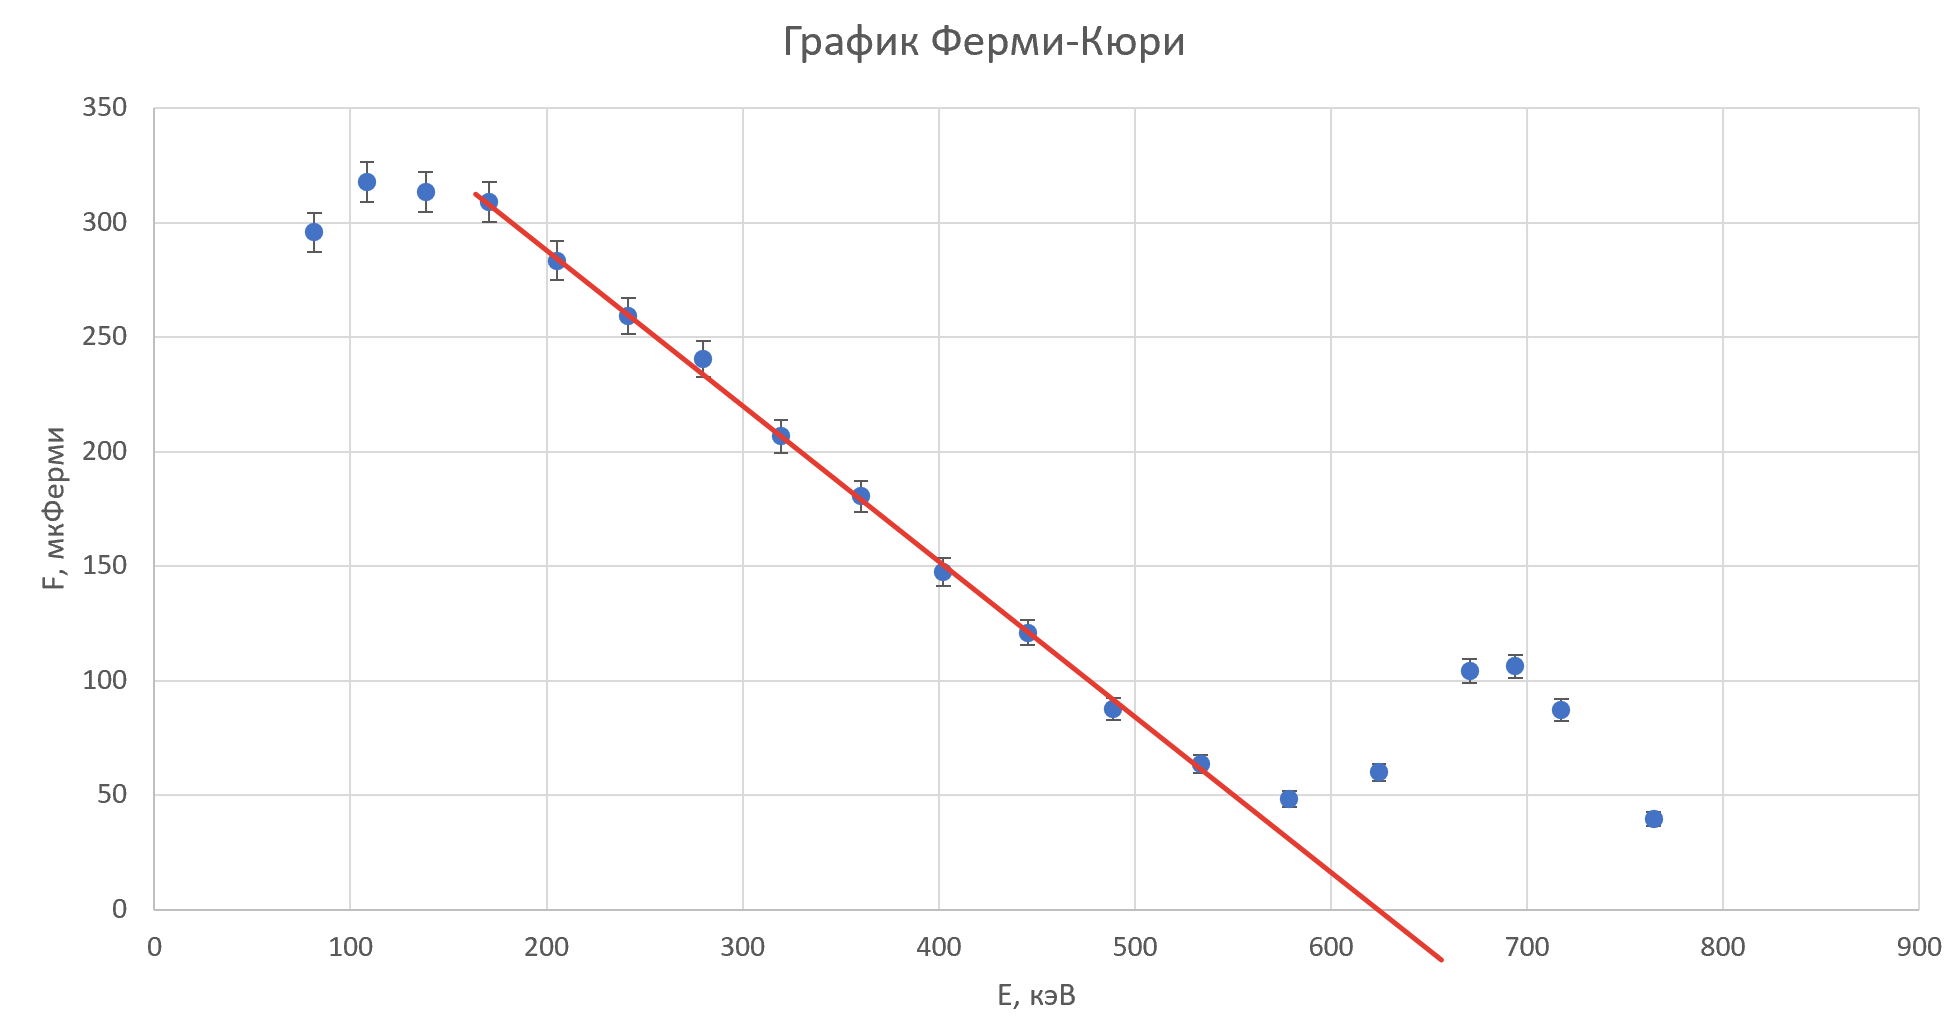
\includegraphics[width=1\textwidth]{bara.png}
	\label{fig:boiler}
\end{figure}
		
		\begin{table}[H]
			\caption{Результаты линейной аппроксимации.}
			\label{table:Emax}
			\begin{tabular}{|c|c|c|}
				\hline
				& $a$, $\text{кэВ}^{-5/2}$ & $\text{кэВ}^{-3/2}$ \\ \hline
							Величина    & -0,748                                                        & 467                                                                     \\ \hline
							Погрешность & 0,018                                                         & 9                                                                       \\ \hline
						\end{tabular}
		\end{table}
		Ясно, что $E_m = - \frac{b}{a}$ и $\sigma_{E_m} = E_m \sqrt{\left(\frac{\sigma_a}{a}\right)^2 + \left(\frac{\sigma_b}{b}\right)}$, откуда $E_m =(620 \pm 20) \ \text{кэВ}.$








%\begin{figure}[!h]
%	\centering
%	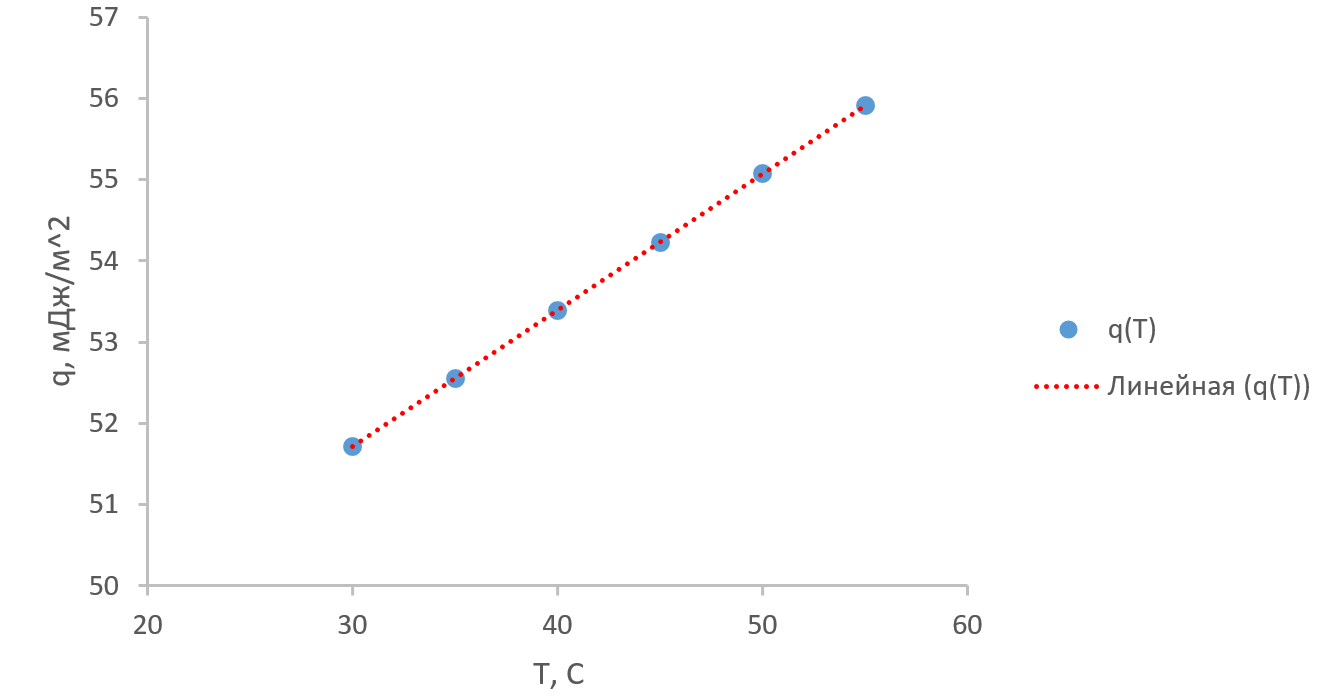
\includegraphics[width=1\textwidth]{2023-02-23_22-23-59.png}
%	\label{fig:boiler}
%\end{figure}

\section{Вывод}

В ходе лабораторной работы с помощью магнитного спектрометра мы исследовали энергетический спектр $\beta$-частиц при распаде ядер $^{137}$Cs. Калибровку спектрометра осуществили по энергии электронов внутренней конверсии.
	
	Анализ графика (рис.~\ref{fig:spectre2}) показывает, что точки купола достаточно хорошо приближаются параболой. Такой вид зависимости согласуется с теоретической. Конверсионный же пик оказывается можно приблизить Гауссовым распределением. Заметим, что в окрестности нуля спектр положителен -- эти точки требуют повторного измерения.
	
	Также мы определили максимальную энергию $E_m = 620$ кэВ вылетающих электронов при $\beta$-распаде ядря $^{137}$Cs методом Ферми-Кюри  с ошибкой в 3\%.


\section{Ресурсы}

Расчет по МНК: метод-наименьших-квадратов.рф


\end{problem}
\end{document}